\documentclass[landscape,a0paper,fontscale=0.32]{baposter}

\graphicspath{{images/}}

\definecolor{dkist1}{RGB}{252,164,30}
\definecolor{dkist2}{RGB}{234,109,28}
\definecolor{dkist3}{RGB}{12,36,113}

\usepackage{fontspec}
% \setmainfont[Ligatures=TeX]{Georgia}
\setsansfont{Roboto}
\setmonofont{Source Code Pro}
\renewcommand{\familydefault}{\sfdefault}

\usepackage{minted}
\setminted[pycon]{autogobble}
\setminted[python]{autogobble}

\begin{document}

\begin{poster}{
 % Show grid to help with alignment
 grid=false,
 % Column spacing
 colspacing=0.7em,
 % Color style
 borderColor=dkist1,
 headerColorOne=dkist2,
 headerFontColor=dkist3,
 % Format of textbox
 textborder=faded,
 % Format of text header
 headerborder=open,
 headershape=rectangle,
 headershade=plain,
 headerheight=0.12\textheight,
 headerfont={\bfseries},
 background=none
 }
 % Eye Catcher
 {
   
\includegraphics[height=0.08\textheight]{dkistlogo.jpg}
 }
 % Title
 {\sc\Huge User Tools for Level 1 DKIST Data}
 % Authors
 {Stuart J. Mumford$^{2,1}$, Fraser Watson$^{1}$, Alisdair Davey$^{1}$\\
 {\footnotesize{1. National Solar Observatory, 2. University of Sheffield}}}
 % University logo
 {
 
\includegraphics[height=0.08\textheight]{dkistlogo.jpg}
 }
 

 
\begin{posterbox}[name=intro,column=0,row=0,span=2]{DKIST Level 1 Data}

  The DKIST Data Centre will be providing level one calibrated data for download
  by the scientific community. In addition to this a set of Python tools are
  being developed to facilitate the use of these data.

  The main features of the user tools will be:
  \begin{itemize}
  \item Dataset search.
  \item Dataset download.
  \item Loading of datasets.
  \item Providing coordinate aware representation of datasets.
  \item Enabling the use of the Scientific Python ecosystem on DKIST level 1
    data.
  \end{itemize}

  
\end{posterbox}

\begin{posterbox}[name=dataset,column=0,row=0,span=1,below=intro]{DKIST Datasets}

  Level 1 DKIST data will be provided as ``datasets'' which divide the data up
  into observations from one instrument and one pass band from one observing
  program.

  These datasets will be divided into many individual FITS files, such that each
  is a single ``calibrated frame'', for example for the VISP slit spectrograph
  each FITS file would be a two dimensional space-wavelength array. This means
  every dataset will be comprised of many tens or hundreds of thousands of FITS
  files.

  One of the primary functions of the user tools is to expose these individual
  frames as a contiguous cube without rewriting the data or having to open the
  files until the array values need to be read.
  
  \begin{center}
    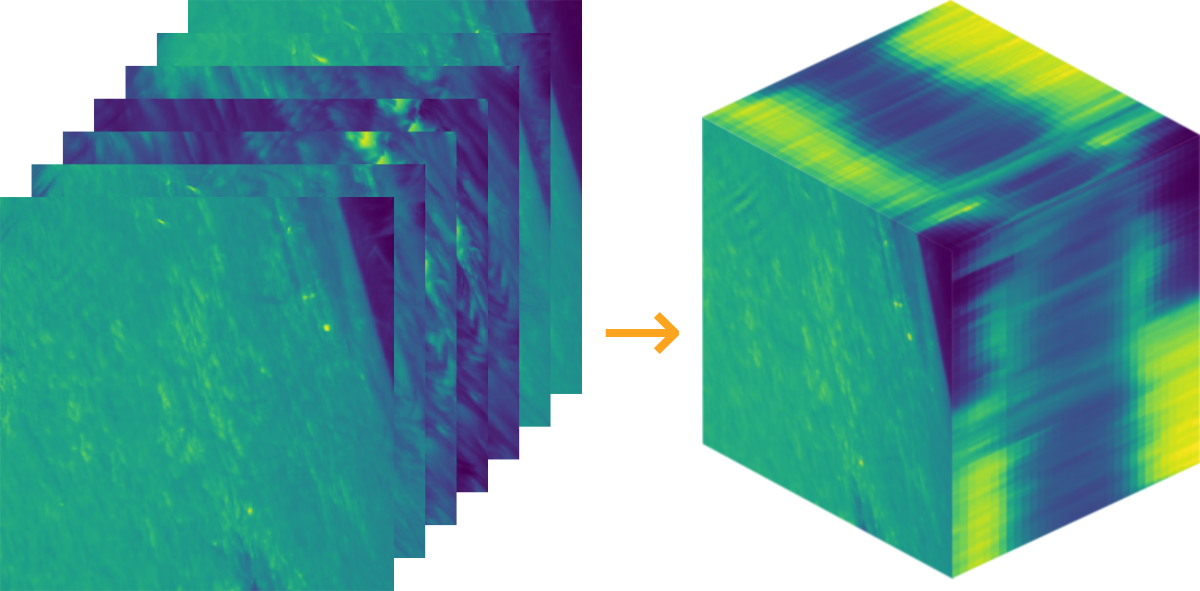
\includegraphics[width=0.75\textwidth]{sequence_and_cube.png}\\[0.4em]
  \end{center}

  To make this more efficient an Advanced Scientific Data Format (asdf) file
  containing all the metadata is provided for each dataset. This asdf file
  contains:
  \begin{itemize}
    \item The ordering information for the FITS files.
    \item A copy of all the FITS headers for all files in the dataset.
    \item A World Coordinate System for the whole reconstructed dataset.
    \item Some additional metadata about the dataset.
  \end{itemize}
  
\end{posterbox}

\begin{posterbox}[name=dask,column=1,row=0,span=1,below=intro]{Dask}
  
  Dask is a Python library for larger than memory and distributed computation.
  The DKIST user tools are utilising dask as a core component to enable the on
  demand loading of data from many FITS files. Representing the dataset as a Dask
  array also provides users lots of potential for parallel computation on a
  variety of hardware from laptops to HPC and cloud computing.

  The Level 1 DKIST data constructs a multi-dimensional array of all the frames
  in a dataset reading the metadata from the datasets asdf file.
  
  \begin{minted}[fontsize=\small]{pycon}
    >>> arr = arr[2:-2]
    >>> arr = np.min(arr, axis=0)
    >>> arr.visualize(optimize_graph=False)
  \end{minted}

  \begin{center}
    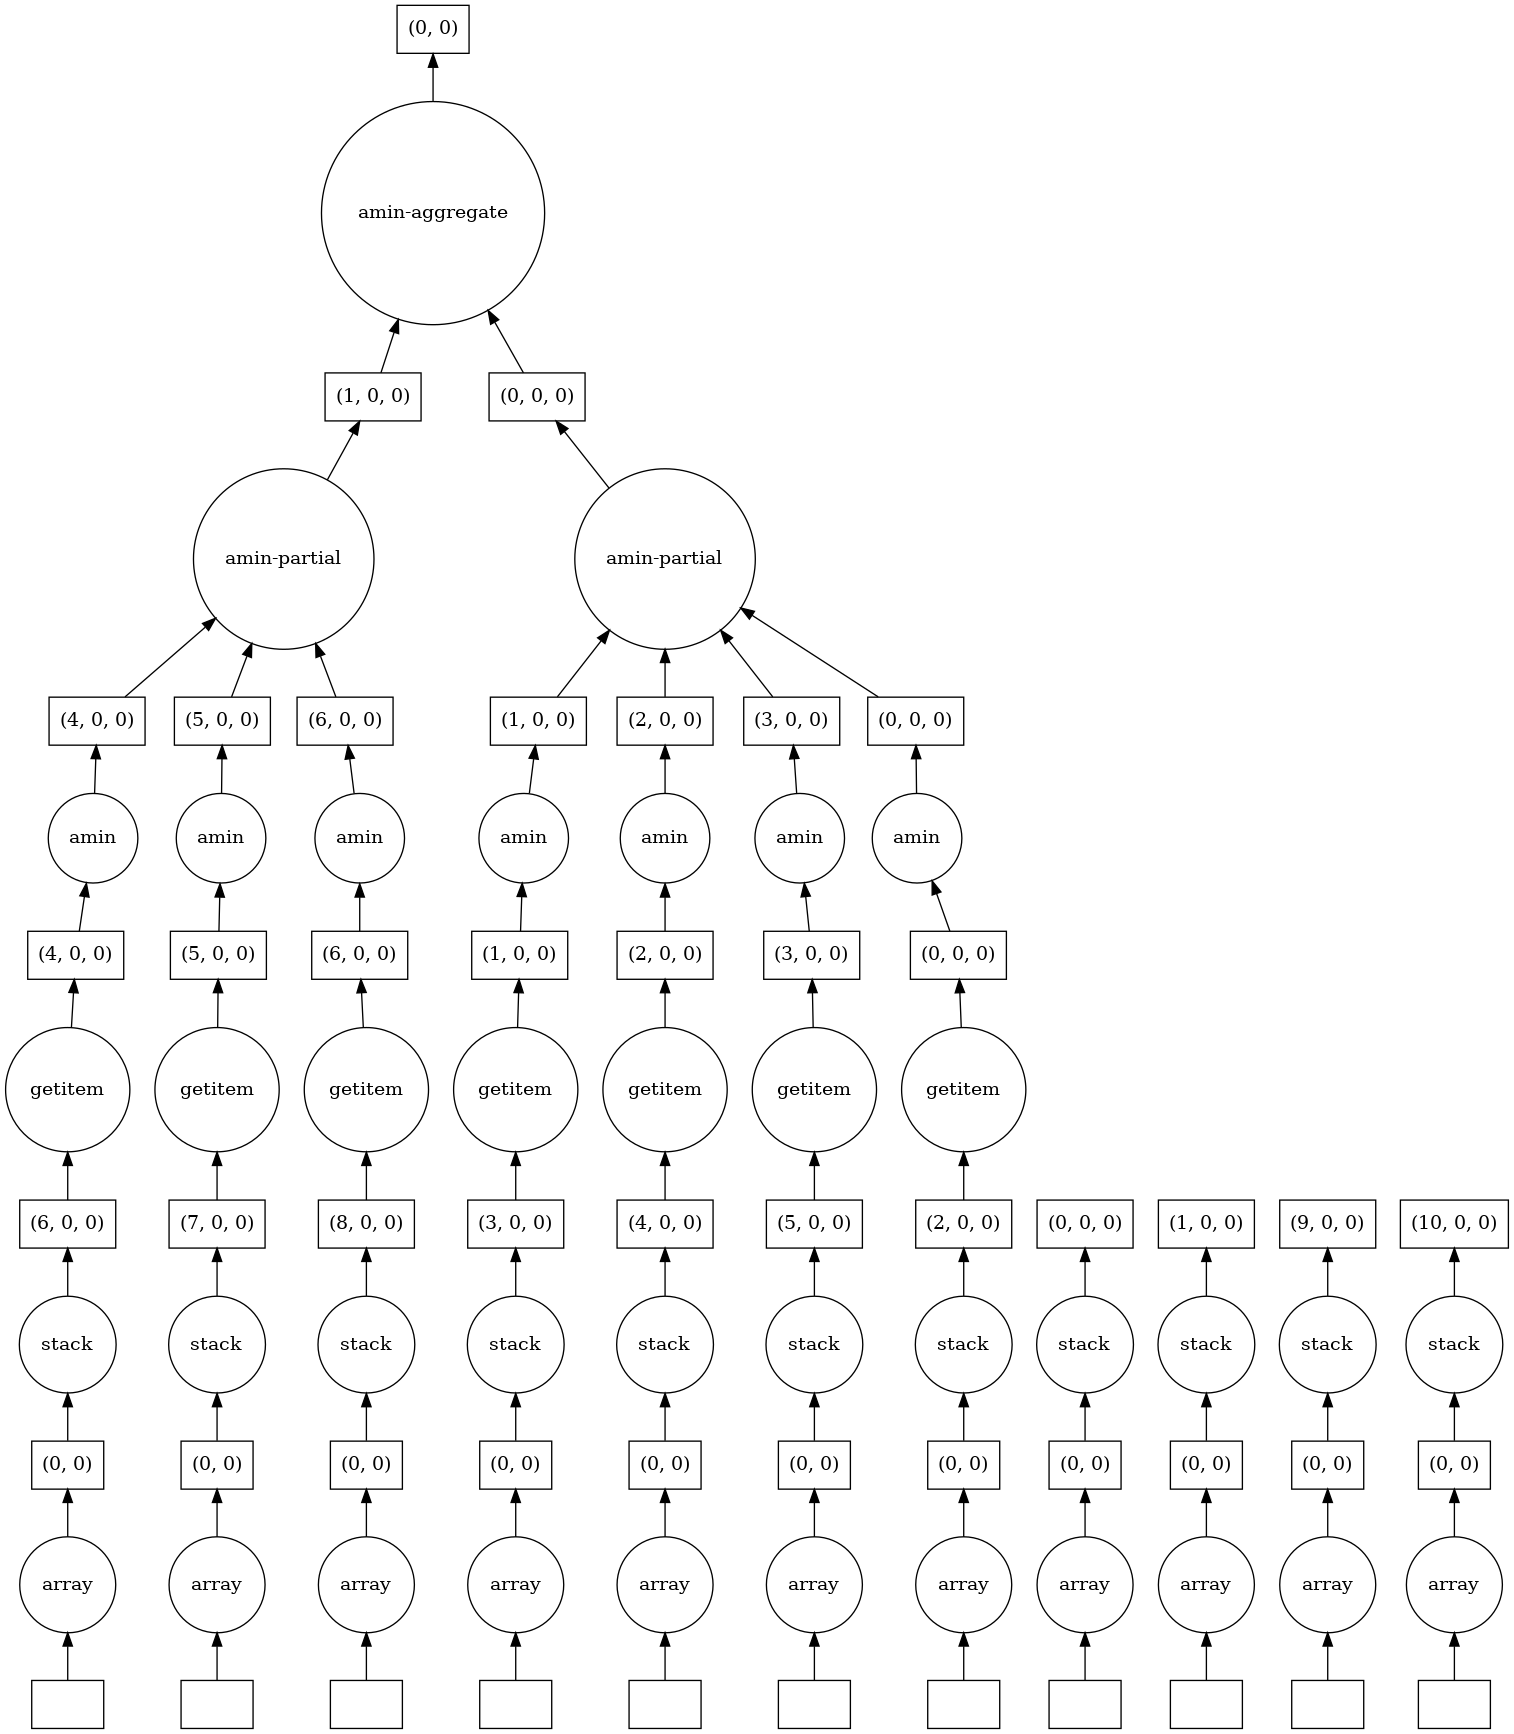
\includegraphics[width=0.6\textwidth]{mydask.png}
  \end{center}

  As shown above, when doing operations on a Dask array, a graph of operations
  is generated, and only when the values of array are required is the graph
  executed. This means that complex operations can be done on a large distributed,
  multi-dimensional dataset, but then the computation can only be done on the
  minimum number of frames at visualisation or analysis time.

\end{posterbox}
 
\begin{posterbox}[name=dataset,column=2,row=0,span=2]{Loading a Dataset}

  The user tools load datasets from asdf files. If the FITS files referenced
  by the asdf file are not present, the dataset can still be loaded and the
  metadata explored.
 
  \begin{minted}[fontsize=\small]{pycon}
    >>> from dataset import Dataset

    >>> ds = Dataset.from_asdf("VTF_20450812T090801.asdf")
    >>> ds
    <dkist.dataset.dataset.Dataset object at 0x7f3245c965c0>
    dask.array<stack, shape=(4, 128, 19, 966, 980), dtype=float32, chunksize=(1, 1, 1, 966, 980)>
    WCS<pixel_axes_names=(stokes, scan number, wavelength position, spatial y, spatial x),
        world_axes_names=(stokes, time, wavelength, latitude, longitude)>
  \end{minted}

  This facilitates the inspection and subsetting of the dataset before having to
  transfer the large arrays. This can be used to only transfer subsets of the
  whole dataset, for example, only Stokes I or a specific time window. Only
  whole FITS files can be transferred as there is no processing before download
  at the data center.

  In the example below we select the 0th stokes profile (I) and the 50th
  wavelength scan from the dataset:
  
  \begin{minted}[fontsize=\small]{pycon}
    >>> partial = ds[0,50]
    >>> partial
    <dkist.dataset.dataset.Dataset object at 0x7f1a40215c88>
    dask.array<getitem, shape=(19, 966, 980), dtype=float32, chunksize=(1, 966, 980)>
    WCS<pixel_axes_names=(wavelength position, spatial y, spatial x),
        world_axes_names=(wavelength, latitude, longitude)>
  \end{minted}

  This subset can then be downloaded, only transferring 19 FITS files out of a
  total of 9728.

  \begin{minted}[fontsize=\small]{pycon}
    >>> partial.download()
  \end{minted}

  
\end{posterbox}

\begin{posterbox}[name=scipy,column=2,row=0,span=1,below=dataset]{Plotting}

  A dataset object is able to display a summary plot for all dimensionalities of
  data. Here we plot our original five dimensional dataset, and three sliders
  are displayed, for wavelength, time and stokes profile.

  \begin{minted}[fontsize=\small]{pycon}
      >>> ds.plot()
  \end{minted}

  \begin{center}
    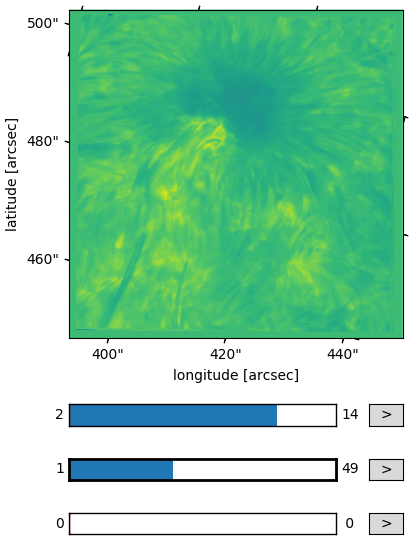
\includegraphics[width=0.65\textwidth]{5d-animator.png}
  \end{center}
  
\end{posterbox}

\begin{posterbox}[name=scipy,column=3,row=0,span=1,below=dataset]{Scientific Python}

  The Scientific Python ecosystem is comprised of a large number of packages
  which specialise in different functionality. The objective of the DKIST user
  tools is to enable the use of this ecosystem with DKIST data.
  
  \includegraphics[width=0.98\textwidth]{scipy-stack.png}\\[0.1em]

  The DKIST user tools uses a large number of these different packages, to
  provide interoperability with the whole ecosystem the key packages used are Dask
  for the array, matplotlib for visualisation, SunPy and Astropy for coordinate
  transformations and units, and gWCS for representation of the world coordinates.

\end{posterbox}

\end{poster}
\end{document}